\section{Scan Konvertierung}

\subsection{Linie Rastern}

\textit{Eine Linie von $(x_0, y_0)$ nach $(x_1, y_1)$ rastern. Da in Pixel konvertiert werden muss. Methoden:}

\begin{itemize}
    \item \textit{Brute Force; über jeden Pixel und runden}
    \item \textit{Brute Force inkrementell (DDA); $y_{i+1} = m * x_{i+1) + B = y_i + m}$,
          Nachteil Gleitkommazahlen und Runden (aufwändig)}
    \item \textit{Mittelpunktschema; Nächsten Punkt wird Kalkuliert durch if / else}
\end{itemize}

\subsection{Mittelpunktschema}

\textit{Ist eine inkrementelle methode zum Rastern. Mittelpunkt
wird betrachtet um nächsten Punkt zu finden. ($M = (x_i+1, y_i+\frac{1}{2})$, $E = (x_i+1, y_i)$, $NE = (x_i+1, y_i+1)$)}\\

$D_x = x_1 - x_0$; \\
$D_y = y_1 - y_0$; \\
$D_E = 2 * D_y$; \\
$D_{NE} = 2 * (D_y - D_x)$; \\
$d = 2*D_y - D_x$; \\
$y = y_0$ \\

\textit{
    Für jeden nächsten $d$ Wert, wenn $d <= 0$,
    dann $d = d + D_{NE}$ ansonsten $d = d + D_{NE}$ und $y$ inkremenrieren.
    Jeweils den Punkt $P(x,y)$ zeichnen. $x$ jedesmal inkrementieren.
}

\subsection{Kreis Rastern}

\textit{Selbe Methode wie bei den Linien kann für Kreise angewendet werden.}

\subsection{Mittelpunktschema Kreis}

\textit{Funktion für Kreis: $F(x,y) = x^2 + y^2 - R^2$}\\

$x = 0$\\
$y = R$\\
$d = 1 - R$\\
$D_{E} = 2*x + 3$\\
$D_{NE} = 2*(x-y)d + 5$\\

\textit{
    Für jeden nächsten $d$ Wert wiederholen bis $y > x$, wenn $d < 0$,
    dann $d = d + D_{E}$ ansonsten $d = d + D_{NE}$ und $y$ dekrementieren.
    Jeweils den Punkt $P(x,y)$ zeichnen. $x$ jedesmal inkrementieren.
}

\subsection{Regionen füllen}

\textit{Entweder durch 4-er oder 8-er zusammenhang definiert}

\begin{tabular}{cl}
    \multirow{3}{*}{
        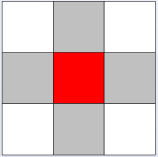
\includegraphics[width=0.05\textwidth]{assets/region-filling-4.png}
    } & \\
    & \textit{4-er Zusammenhang} \\
    & \\
\end{tabular}
\begin{tabular}{cl}
    \multirow{3}{*}{
        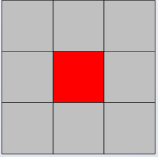
\includegraphics[width=0.05\textwidth]{assets/region-filling-8.png}
    } & \\
    & \textit{8-er Zusammenhang} \\
    & \\
\end{tabular}

\subsection{FloodFill}

\textit{Füllen durch selben abfrage ob selbe Farbe (Photoshop Zauberstab)}

